\documentclass[runningheads]{llncs}

\usepackage{graphics}
\usepackage{url}

\newcommand{\ccorn}{\mbox{C-CoRN}}
\newcommand{\coq}{Coq}
\newcommand{\coqdoc}{\texttt{coqdoc}}
\newcommand{\fta}{FTA}
\newcommand{\weg}[1]{}
\newcommand{\nth}{$n^{\mathrm{th}}$}

\author{Lu\'\i s Cruz-Filipe\inst{1,2} \and Herman Geuvers\inst{1} \and Freek Wiedijk\inst{1}}
\institute{NIII, Radboud University Nijmegen\and Center for Logic and Computation, Lisboa\\ \email{lcf|herman|freek@cs.kun.nl}}

\authorrunning={L. Cruz-Filipe, H. Geuvers, F. Wiedijk}

\title{C-CoRN, the Constructive Coq Repository at Nijmegen}
 
\begin{document}
\maketitle
\begin{abstract}
We present \ccorn, the Constructive Coq Repository at Nijmegen. It
consists of a mathematical library of constructive algebra and
analysis formalized in the theorem prover Coq. We
explain the structure and the contents of the library and we discuss
the motivation and some (possible) applications of such a library. 

The development of \ccorn\ is part of a larger goal to design a
computer system where `a mathematician can do mathematics', which
covers the activities of defining, computing and proving. An important
proviso for such a system to be useful and attractive is the
availability of a large structured library of mathematical results
that people can consult and build on.  \ccorn\ wants to provide such a
library, but it can also be seen as a case study in developing such
a library of formalized mathematics and deriving its requirements. As
the actual development of a library is very much a technical activity,
the work on \ccorn\ is tightly bound to the proof assistant Coq.
\end{abstract}

\section{Introduction\label{introduction}} 
A repository of formalized constructive mathematics \cite{ccorn} in
the proof assistant Coq~\cite{coqmanual} has been constructed over the
last five years at the University of Nij\-megen. This is part of a
larger goal to design a {\em mathematical assistant\/}: a computer
system in which a mathematician can do mathematics. This covers the
activities of defining (theory development), computing (programming)
and proving (proof development), but ideally also editing of
mathematical documents and presentation of mathematics.  In such a
computer system, the mathematics would obviously have to appear in a
{\em formalized\/} form, i.e.\ as expressions in some formal
language. The process of going from the informal (paper) mathematics
to the mathematics that can be understood and manipulated by a
computer (program) is called {\em formalization}.

\weg{
Thanks to this we now have a pretty good idea of what such
a system should look like and how it should be made; through
foundational and experimental research we want to contribute ideas and
results that support the actual development of such a system in the
future.
}

One of the things that is very important for such a `mathematical
assistant' to be used is the availability of a large and usable
library of basic results.  A library will make it attractive for
potential users to experiment with the system and to contribute
results to its repository. Such a repository should not be just a
huge collection of proved results (including the `proof scripts' that
are input for the proof assistant to carry out the proof). In our
view, a library of formalized mathematics should be:
\begin{description}
\item[Accessible:] one should be able to get a fairly fast overview 
of what's in it and where to find specific results;
\item[Readable:] once one has come down to the basic objects like 
definitions, lemmas and proofs, these should be presented in a
reasonable way;
\item[Coherent:] results about a specific theory should be grouped 
together and theories extending others should be defined as such;
\item[Extensible:] contributions 
from other researchers should be easy to include.
\end{description}
How can one make such a (large) coherent library of formalized mathematics? 
Ideally, this should also be independent of the Proof Assistant one is
working with, but right now that cannot be done.
Several other projects deal with this question. The Mowgli
project \cite{mowgli} aims at devising system-independent tools for
presenting mathematics on the web. The OpenMath \cite{openmath} and OMDoc
\cite{OMDoc} standards aim at exchanging mathematics across different
mathematical applications, which is also one of the aims of the
Calculemus project \cite{calculemus}. This may eventually lead to ways
of sharing mathematical libraries in a semantically meaningful way
that preserves correctness, but this is not possible yet
(an exception is NuPRL, which can use HOL results \cite{hol-to-nuprl}).

So, to experiment with creating, presenting and using such a library,
one has to stick to one specific theorem prover, and already there
many issues come up and possible solutions can be tested. We have
chosen to use the Coq Proof Assistant, because we already were
familiar with it and because we were specifically interested in
formalizing constructive mathematics. 

This paper first describes the backgrounds of \ccorn: its history and
motivation. Then we describe the structure of the repository as it is
now and the methodology that we have chosen to develop it. Finally we
discuss some applications and future developments.

\section{History\label{history}}          
The {\ccorn} repository grew out of the {\fta} project,
where a constructive proof of the Fundamental Theorem of Algebra was
formalized in Coq.  This theorem states that every non-constant
polynomial $f$ over the complex numbers has a root, i.e., there is a
complex number $z$ such that $f(z) = 0$.

One of the main motivations for starting the
{\fta} project was to create a library for basic constructive algebra and
analysis to be used by others. Often, a formalization is only used by
the person that created it (or is not used further at all!), whereas
an important added value of formalizing mathematics -- in our view --
is to create a joint computer based repository of mathematics. For the
{\fta} project, this meant that we did not attempt to prove the theorem
as fast as possible, but that in the proving process we tried to
formalize the relevant notions at an appropriate level of abstraction,
so that they could be reused.

An important condition for the successful use of a library of
formalized mathematics is to have good documentation of the code.
There are two main purposes of documentation:
\begin{enumerate}
\item\label{1}
to show to the world
what has been formalized via a `high level' presentation of the work
(in our case that would be a \LaTeX\ document giving a mathematical
description of the formalized theory);
\item\label{2}
to help the interested
outsider to extend (or change or improve or vary on) the formalized
theory.
\end{enumerate}

\looseness=-1
For (\ref{1}) one wants to produce a \LaTeX\ document that `goes
along' with the formalization. This may be generated from the
formalization (but it is not quite clear whether it is at all possible
to generate something reasonably, and mathematically abstract, from the
very low level formal proof code).  Alternatively -- and this is the
approach followed in the {\fta} project --, this \LaTeX\ file may be
created in advance and then used as a reference for the proof to
formalize.  The goal of the {\fta} project was to formalize an {\em
existing\/} proof and not to redo the mathematics or `tailor' the
mathematics toward the proof assistant. This meant that we started
from an original proof of {\fta}, described in~\cite{geuvers2001},
with lots of details filled in to ease the formalization process.  The
same approach has been followed throughout the rest of {\ccorn}:
existing mathematics is formalized, so the (high-level) mathematical
content corresponds to an existing part of a book or article.

For (\ref{2}), some simple scripts were created in the {\fta} project to be
able to extract from the Coq input files a useful documentation for
outsiders interested in the technical content. However, this was
pretty \emph{ad hoc} and not very satisfactory, and it
was changed in {\ccorn}, as described in Section~\ref{methodology}.

After the {\fta} project was finished, i.e., after the theorem had been
formally proved in Coq, it was not yet clear that it had been
successful in actually creating a usable library, because all people
working with the library until then were part of the project. The only
way to test this would be to let outsiders extend the library.
This is not too easy:
due to the fact that we have tactics implemented in ML
(e.g.\ to do equational reasoning), one cannot use the standard image of Coq and
has to build a custom image first.
Therefore, the first real test only came when the first author
of this paper
started as a new Ph.D.\ student to formalize constructive calculus
(leading to the Fundamental Theorem of Calculus) in Coq. The {\fta}
library turned out to be very usable. Most importantly, there was almost no
need to restructure the library or redefine notions, implying that most of the
basic choices that were made in the {\fta} project worked. (Of course, the
basic library was extended a lot, with new results and new
definitions.)  Hereafter, the library was rebaptized to {\ccorn}, the
Constructive Coq Repository at Nijmegen, since the {\fta} and the work of
the {\fta} project had become only a (small) part of it.

Since then, several people, working both in Nijmegen and elsewhere,
have consulted, used and contributed to \ccorn.
These have found its 
structure (including notations, automation facilities, documentation)
quite useful.


\section{Why {\ccorn}?\label{why}}                  
Formalizing mathematics can be fun. In the process of formalizing, one
discovers the fine structure of the field one is working with and one
gains confidence in the correctness of the definitions and the proofs.
In addition to this, formalizing mathematics can also be useful. We
indicate some of its possible uses:
\begin{description}
\item[Correctness guaranteed:] The formalized mathematics is checked
and therefore the proofs are guaranteed to be correct for all
practical purposes. This can be vital in the realm of software or
system correctness, where one wants to be absolutely sure that the
mathematical models and the results proved about them are correct.
\item[Exchange of `meaningful' mathematics:] That the mathematics is 
formalized means that it has a structure and a semantics within the
Proof Assistant. So a mathematical formula or proof is not just a
string of symbols, but it has a structure that represents the
mathematical meaning and its building blocks have a definition (within
the Proof Assistant). These can in principle be exploited to generate
meaningful documents or to exchange mathematics with other
applications.
\item[Finding mathematical results:] Based on the semantics and the
structure of the formalized mathematics, it should be possible to find
results easier. Querying based on the (meaningful) structure is
already possible (implemented in the Helm system, see
\cite{guidi2003}), but more semantical querying would be welcome. 
This requires adding more meta-data.
\end{description}

The potential uses of formalized mathematics only really become
available if one can share the formalization and let others profit
from it, e.g.\ by making it possible for them to study it, extend it
or use it for their own applications or further development. A key
requirement for this is that the formalized mathematics be presented.
Ordinary (non-computer-formalized) mathematical results are published
in articles, books or lecture notes, and are in that way shared with
other mathematicians or users of mathematics.  Giving a good
presentation of formalized mathematics in practice, though, turns out
to be quite hard. There are various reasons for this:
\begin{description}
\item[Idiosyncrasies of the Proof Assistant:]
When talking to a Proof Assistant, things have to be stated in a
specific way, so the system understands it: definitions have to be
given in a specific format, proofs have a specific form, etc. Moreover,
each Assistant has its own logical foundations (e.g.\ set theory, type theory
or higher order logic), making it easy to express some concepts
(e.g.\ inductive definitions in type theory) and hard to express
others (e.g.\ subsets in type theory). Because of this, mathematical
theory will be defined in a specific way that best fits the
idiosyncrasies of the system at hand. When presenting the formal
mathematics, one would like to abstract from these `arbitrary'
choices.
\item[Verbosity of formalized mathematics:]
To make the Proof Assistant understand (or be able to verify) what the
user means, a lot of details have to be given. By itself, this is
unavoidable (and fine, because we really want the mathematics to be
verified and that doesn't come for free). But in the presentation
phase, one wants to abstract from these finer details and `view' the
mathematics at a higher level. This is not so easy to achieve. Ideally
it would also be possible to use the higher level (less verbose)
mathematics as input for the proof assistant, but that's not easy
either.
\item[Access to the formalized mathematics:]
How does one find a result in the library, how does one get an
overview of the material? One can query the library with syntactic
means, searching a formula of a specific form, as described 
in~\cite{guidi2003}.
This is helpful, but can a useful result still be found if it
occurs in the library in disguise?
Also, if a user knows that a
specific lemma appears in the library, (s)he will want to apply it,
which in a Proof Assistant is done by using its name. But what is the
name of (the proof of) a lemma? One probably doesn't want to clutter
up the names in the presentation of the math, so `logical' naming
conventions come in handy.
\end{description}

To really understand and work on these points, one needs a
`testbed' to experiment with. This was one of the reasons to start
{\ccorn}: to have a library of mathematics that people can really
contribute to, read and work with.

Of course, such libraries already exist. The prominent one is the
Mizar Mathematical Library (MML).  However, Mizar was not good for 
experimenting with a library of formalized mathematics,
because we would not have control over the library: one cannot just
install Mizar and formalize a large library on top of the existing
one. Soon the system gets slow and one has to submit the work to the
Mizar library to have it integrated. Moreover, the Mizar system itself
is not open in the sense that one can program one's own tools (e.g.\
for automation or documentation) on top of it\footnote{Right now,
\ccorn\ is not open either: we want to have `central control' over
the library. But the point we want to make here is that the Proof
Assistant Coq, on which \ccorn\ is based, {\em is\/} open.}.
Another important reason not to choose Mizar was that we were aiming
at a library of {\em constructive\/} mathematics. For all these
reasons, Coq was a good choice, with the drawback that there was only
a very small initial library to begin with. (There are many `Coq
contributions', but they do not form one coherent library as discussed
in Section~\ref{related}.)

The main reason for working constructively is that we want to use our
library, apart from studying how it conducts as a repository, to study
the connections between `conceptual' (abstract) mathematics and
`computational' (concrete) mathematics. The first (conceptual math)
deals with e.g.\ the proof of (and theory development leading to) the
Fundamental Theorem of Algebra, while the second (computational math)
deals with an actual representation of the reals and complex numbers
and the actual root finding algorithm that the {\fta} exhibits. In
this paper we will not elaborate on this any further, but just point
out that this was an important motivation for choosing to work with
Coq. At present work is being done in program extraction from the
\ccorn\ library, and this relies heavily on the fact that the library
is constructive.

\section{Contents\label{contents}}

\ccorn\ includes at present formalizations of significant pieces of
mathematics.  In this section we give an overview of the main
results in the library.
So far everything
has been formalized constructively.  Although we do not exclude adding
non-constructive theorems to the library, working constructively has
some added value, as indicated 
in the previous section.

\weg{
A second reason for restricting to constructive proofs is that
intuitionistic logic is the natural language of the type theory on
which \coq\ is based; therefore it seems nicer to work without adding
extra axioms insofar this is feasible.  Also, adding the principle of
excluded middle to the present-day type theory of \coq\ is not
completely straightforward, as some intuitively obvious forms of it
turn out to be inconsistent.

Finally, all constructive reasoning remains valid when classical reasoning is
allowed; hence a constructive formalization will be, at least in principle,
accepted by a larger audience.
}

The \ccorn\ library is organized in a tree-like fashion.
This structure agrees with the dependencies among the mathematics being
formalized.
In Figure~\ref{fig:tree} the directory structure of \ccorn\ can be seen.
\begin{figure}
%\hfill\scalebox{.35}{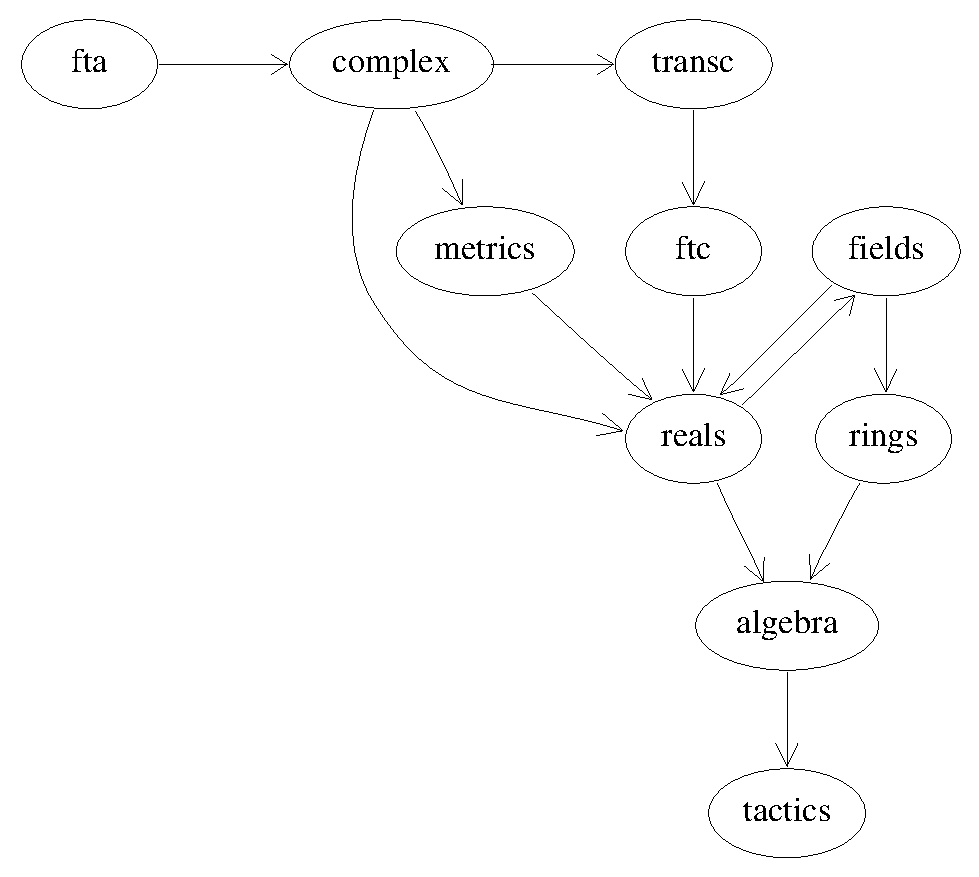
\includegraphics{ccorn-dirs.eps}}\hspace*{\fill}
\hfill\scalebox{.5}{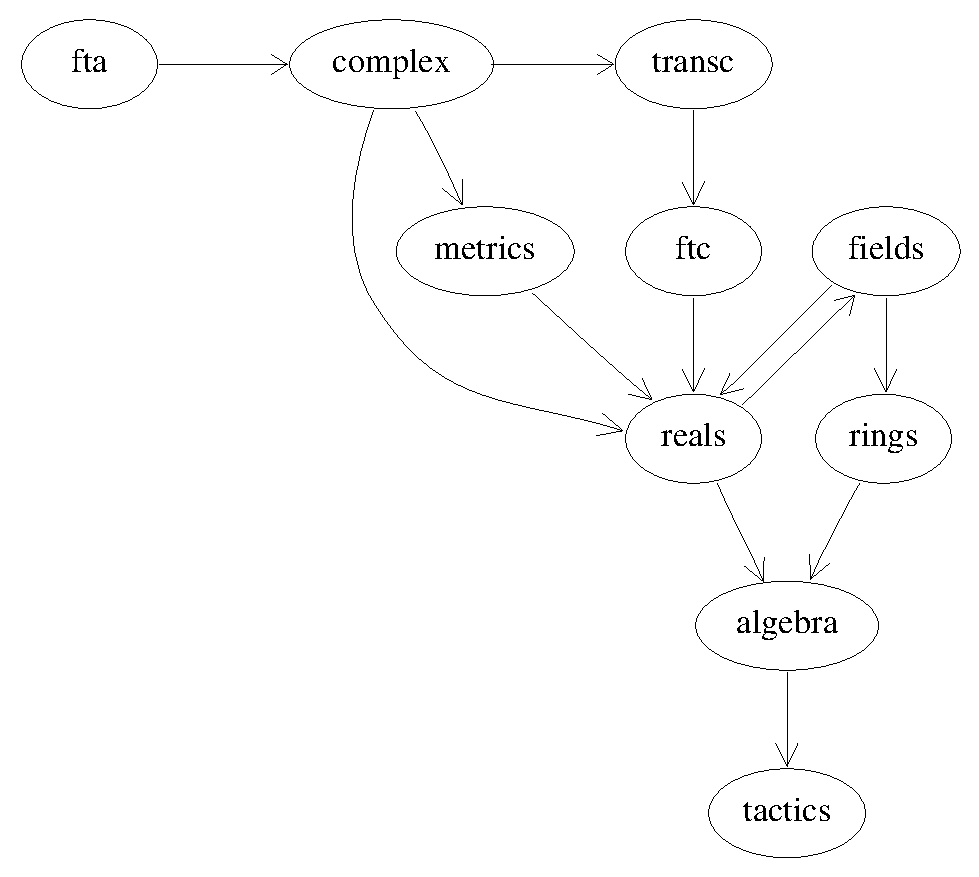
\includegraphics{ccorn-dirs.eps}}\hspace*{\fill}
\caption{Directory structure of \ccorn}
\label{fig:tree}
\end{figure}

At the bottom of {\ccorn} are the tactic files and the Algebraic
Hierarchy, developed in the framework of the {\fta} project. Most of the
tactics are to make equational reasoning easier,
see~\cite{geuvers2000}. In the Algebraic Hierarchy, the most common
algebraic structures occurring in mathematics, such as monoids, rings and
(ordered) fields, are formalized in a cumulative way and their basic
properties are proved.  For reasons discussed in
Section~\ref{methodology}, this formalization proceeds in an abstract
way, described in detail in~\cite{geuvers2002}.
Furthermore, the hierarchy is built in such a way that more
complex structures are instances of simpler ones, i.e.\ all
lemmas which have been proved e.g.\ for groups are inherited by all
ordered fields.

One might argue that tactics should not be part of a library of mathematics
but are `meta-knowledge'.
However in {\ccorn} the tactics are closely related to the lemmas
that they depend on: these cannot be easily separated.
Also lemmas and tactics can be exchanged for each other:
a proof step often can be made either with reference to a lemma (declarative
mathematical knowledge)
or by applying a tactic (procedural mathematical knowledge).
For these reasons we consider tactics to be part of the {\ccorn} library.

Real number structures are defined as complete archimedean
ordered fields.
The \ccorn\ library includes not only a concrete model of the real numbers
(namely, the standard construction as Cauchy sequences of rationals) but also
a formal proof that any two real number structures are equivalent and some
alternative sets of axioms that can be used to define them.
Thanks to these results, it makes sense to work with a generic real number
structure rather than with any concrete one.
This part of the library is described in detail in~\cite{niqui2002}.

Among generic results about real numbers included in the library we point out
the usual properties of limits of Cauchy sequences and the Intermediate Value
Theorem for polynomials, which allows us in particular to define \nth\ roots
of any nonnegative number.

At this point the library branches in various independent directions.

One of the branches consists of the rest of the original {\fta} library, which
contains the definition of the field of complex numbers and a proof of the
Fundamental Theorem of Algebra due to M.\ Kneser;
this work is discussed in~\cite{geuvers2001}.
Other important results in this part of the library include the definition
of important operations on the complex numbers (conjugation, absolute value
and \nth\ roots) and their properties.

The second main branch deals with a development of Real Analysis
following~\cite{bishop1967}.
Here, properties of real valued functions are studied, such as continuity,
differentiability and integrability.
Several important results are included, among which Rolle's Theorem, Taylor's
Theorem and the Fundamental Theorem of Calculus.
Also, this segment of the library includes results allowing functions to be
defined via power series; as an application, the exponential and trigonometric
functions are defined and their fundamental properties are proved.
Logarithms and inverse trigonometric functions provide examples of function
definition via indefinite integrals.

A separate branch of the library, currently in its initial stage of
development, deals with topological and metric spaces.
At present this part of the library is very small; it includes simple
properties of metric spaces, as well as a proof that the complex numbers
form a metric space.

The sizes of the different parts of the \ccorn\ library are shown in
Figure~\ref{fig:contents}.
\begin{figure}
\hfill\begin{tabular}{l|c|c}
 Description                          & Size (Kb) & \%\ of total \\ \hline
 Algebraic Hierarchy (incl.\ tactics) & 533       & 26.4         \\
 Real Numbers (incl.\ Models)         & 470       & 23.3         \\
 FTA (incl.\ Complex Numbers)         & 175       &  8.7         \\
 Real Analysis (incl.\ Transc.\ Fns.) & 842       & 41.6         \\ \hline
 Total                                & 2020      & 100          \\ \hline
\end{tabular}\hspace*{\fill}
\caption{Contents and size of \ccorn\ (input files)}
\label{fig:contents}
\end{figure}
This data does not include the files dealing with metric spaces, as these are
still in an early stage of development, nor those dealing with applications to
program extraction, which will be discussed in Section~\ref{applications}.

\section{Methodology\label{methodology}}

In order to successfully pursue the goal of formalizing a large piece of
mathematics, it is necessary to work in a systematic way.
In this section we look at some of the general techniques that are used to
make the development of the \ccorn\ library more fluent.

We will focus on four main aspects:
\begin{description}
\item[Documentation:] In order to be usable, a library needs to have a good
documentation that allows the user to quickly find out exactly what results
have been formalized, as well as understand the basic notations, definitions
and tactics.
\item[Structuring:] Another important issue is the structure of the library.
We feel that lemmas should be somehow grouped according to their mathematical
content rather than to any other criterion; e.g.\ all lemmas about groups
should be put together in one place, all lemmas about order relations in
another, and so on.
A related aspect is how to name lemmas.
Experience shows that following some simple rules can make the process of
looking for a particular result both easier and faster.
\item[Abstract approach:] \ccorn\ aims at generality.
This suggests that mathematic structures (e.g.\ real numbers) be formalized in
an abstract way rather than by constructing a particular example and working
on it.
We will examine some of the consequences of this style of working.
\item[Automation:] Finally, any successful theorem-proving environment must
have at least some automation, otherwise the proving process quickly becomes
too complex.
We give an overview of the specific tactics that were developed for \ccorn\ 
and show how they help in the development of the library.
\end{description}

\subsection*{Documentation}

Providing a good documentation for the formalized library in parallel
with its development was a central preoccupation from the beginning of
the {\fta} project.  In fact, having a human-readable description of
what has been formalized can be very useful in communicating not only
content but also ideas, notations and even some technical aspects of
the formalization process.

Such a documentation should at any given moment reflect the state of
the library, and as such should be intrinsically linked to the script
files.  (This is also the idea behind Knuth's `Literate Programming'.
Aczel and Bailey use the term `Literate Formalization'
for this method applied to formalized mathematics \cite{bailey1998}.)
At present, \coq\ provides a standard tool, called \coqdoc\ 
(see~\cite{coqdocmanual}), that automatically generates postscript and
\texttt{html} documentation from the \coq\ input files.  Additional
information can be introduced in the documentation via comments in the
script file.

Ideally the documentation should be one with the script files; however
this is not the situation in \coq.  In this system the standard way to
generate documentation for a library is using \coqdoc, and this is the
way we do it in \ccorn.
The \ccorn\ documentation includes all definitions, axioms and
notation as well as the statements of all the lemmas in the library,
but no proofs: being meant as \emph{documentation}, rather than
\emph{presentation} of the library, the presence of long
and incomprehensible proof scripts in the documentation would
undermine its purpose.
For the same reason, tactic definitions are omitted from the documentation,
but not their description: although the actual code is not presented, the
behavior of the existing \ccorn\ specific tactics is explained as well as how
and when they can be used.

In the \texttt{html} version, hyperlinks between each occurrence of a term and
its definition allow the users to navigate easily through the documentation,
being able to check quickly any notion they are not familiar with.

\subsection*{Structuring}

There are several ways that the lemmas and files in a library of
formalized mathematics can be organized.  The current trend in most
major systems, as discussed in Section~\ref{related}, seems to be
adding individual files to the library as independent entities and
seldom if ever changing them afterward (except for maintenance).
However, \ccorn\ is intended as a growing system upon which new
formalizations can be made.
The approach above described directly conflicts with this purpose, for it
typically leads to dispersion of related lemmas throughout the library and
unnecessary duplication of work.

For this reason, lemmas in {\ccorn} are organized in files according
to their statements and files are distributed in directories
according to their subjects.
Thus, different areas of mathematics appear in different directories and
different subjects within one area will be different files in the same
directory. 

The disadvantage of this approach is that it requires some form of central
control over the repository:\label{contradictions} after an
extension, the library has to be reconsidered to put the definitions
and lemmas in the `right' place. This may become problematic if many
files are contributed within a short time.
Presently the responsibility for maintaining different parts of {\ccorn}
is distributed among different people: when a subject becomes extensively
represented in the library, we encourage the developers of that subject to
take responsibility for it.
In this way we do not restrict the control of the library to a small group
of people or a confined geographical location, but we manage to keep its
unity.
We also hope that new users will feel motivated to work in {\ccorn} and
extend it.

No part of the library is, strictly speaking, immutable: new
lemmas can be added at any time to existing files, if they are felt to belong
there.
In this way, new lemmas then become immediately available to other users.
In practice, though, the lower in the tree structure of Figure~\ref{fig:tree}
a file is, the less often it will be changed.

Coupled with this method of working, the documentation system described above
makes looking for a particular statement a simpler process than in most of the
systems the authors are acquainted with.
But in addition to this, naming conventions are adopted throughout
\ccorn\ that allow experienced users to find a specific lemma even
more quickky without needing to consult the documentation.
These naming conventions are too specific to be explainable in a
short amount of space; the interested reader can find them throughout
the \ccorn\ documentation.

\subsection*{Abstract Approach}

One finds two approaches to formalizing algebraic operations.  On the
one hand one just has concrete types for various number structures,
like the natural numbers, the integers, the real numbers and the
complex numbers, and for each of those one defines a separate set of
arithmetical operations.  On the other hand -- which is the approach
that is followed in {\ccorn}, as described in~\cite{geuvers2002} --
one can have a hierarchy of the commonly appearing algebraic
structures in mathematics, such as groups, rings, fields and ordered
fields, and then instantiate these to specific number structures.  In
this approach the theory of the real numbers will not refer to a
specific type of real numbers, but just to a type of `real number
structure', which later can be instantiated to a concrete
model\footnote{In {\ccorn} this algebraic hierarchy is formalized
using record types, making the abstract structures first class
citizens (types) of the system. Another way to proceed (which wasn't
available at the time {\ccorn} was started) would be to use Coq's
modules.}.

This second approach has advantages and disadvantages.
An advantage is that the theory that is developed for a certain
structure is maximally reusable.
For example, the group properties can be reused for the integers, 
the rational numbers, the real numbers, polynomials, vectors
in a vector space, and so on.
In our abstract approach each of these structures will
be just an instance of the already existing algebraic type of
groups,
and the laws that were proved for this type will be immediately available.
In the first approach the same theory has to be developed over and
over again every time a new structure with the same
algebraic properties is defined.

Another advantage is that the same notation will be used
for the same algebraic operation.
This is especially useful in a system that has no overloading,
like Coq.
For instance, in the first approach one has different additions
on natural numbers, integers, real numbers,
while in {\ccorn} all of these are simply written as \texttt{(x[+]y)}.

A third advantage is that the development of the theory will
more closely follow the development of algebra in a mathematical
textbook.

The main disadvantage of the abstract approach is that
the terms that occur in the formalization are usually much bigger,
because they have to refer to the specific structure used.
Also, because of the hierarchy of the types of algebraic
structures, there will be functions needed in the terms to get to the
right kind of algebraic structure.
This is not a problem for the user, since
all these operations are implicit:
the specific structure is generally an implicit argument,
while the functions that map algebraic structures are
coercions.
But internally these terms are big,
so it slows down the processing of the formalization by Coq.

Another slight disadvantage of this approach is that
sometimes proofs can be less direct than in the case where
all functions are concretely defined.
This also affects program extraction.
For instance, if one knows that one is dealing with the
rational numbers, a proof might be possible that gives
a much better extracted program.
In the case that one has to give a proof from an abstract specification,
this optimization might not be available.

\subsection*{Automation}

An important part of the \ccorn\ library consists in tools designed to aid in
its own development.
Together with definitions, notations and lemmas, several automated tactics are
defined throughout \ccorn.

These tactics vary in complexity and in their underlying mechanism.
Thus, there are several tactics based on \coq's \texttt{Auto} mechanism, which
simply performs Prolog-style depth-first search on a given collection of
lemmas.
Each tactic is designed for a specific subject, such as 
equational reasoning in different algebraic structures (\texttt{Algebra}) or proving
continuity of real-valued functions
(\texttt{Contin}).

Other tactics base themselves on the principle of reflection to tackle wider
classes of problems in a more uniform and more efficient way.
We mention \texttt{rational}, described in detail in~\cite{geuvers2002}, which
provides proofs of equalities in rings or fields, but can solve a much larger
class of goals than \texttt{Algebra}; and \texttt{Deriv}, described
in~\cite{cfilipe2002}, a reflective tactic which can prove goals of the form
$f'=g$ when $f$ and $g$ are real-valued (partial) functions.
Although tactics based on reflection are usually more powerful than those based
on \texttt{Auto}, they are also more time consuming when the goals are simple
and usually cannot infer as much information from the context as the latter.

Finally, an interface for equational reasoning is also provided via the
\texttt{step} tactic.
This tactic allows the user to replace a goal of the form $R(a,b)$,
where $R$ is a relation and $a$ and $b$ have appropriate types, by
either $R(c,b)$ or $R(a,c)$, where $c$ is a parameter given by the
user.  This tactic looks through a database of lemmas that state
extensionality of (various types of) relations, and chooses the one
which applies to $R$. Then it applies either \texttt{Algebra} or
\texttt{rational} to prove the equational side condition generated by
the lemma.

The \texttt{step} tactic has been generalized to work in a
much wider domain than that of {\ccorn} and is now included in the
standard distribution of \coq.

\section{Applications\label{applications}}

Besides the direct interest of formalizing mathematics \emph{per se}, there
are some interesting applications that are either being explored at present
or are planned for the near future.

One of the consequences of working constructively, and therefore without any
axioms, is that, according to the Curry-Howard isomorphism, every proof is
an algorithm.
In particular, any proof term whose type is an existential statement is also
an algorithm whose output satisfies the property at hand.
This allows us to obtain correct programs for free, which is an interesting
possibility.

In \coq\ there is an extraction mechanism available that readily transforms
proof terms into executable ML-programs (see~\cite{letouzey2003}).
Marking techniques are used to reduce the size of extracted programs
significantly, as most of the information in the proofs regards
\emph{correctness} rather than \emph{execution} of the algorithm and
can be safely removed.
In~\cite{cfilipe2003} it is described how this extraction mechanism was used
to obtain, from the formalized proof of the Fundamental Theorem of Algebra,
an algorithm that computes roots of non-constant polynomials.
At the time of writing the extracted program is too complex and does not
produce any output in a reasonable amount of time; but the same method has
been used to produce a \emph{correct} program that can compute $150$ digits of
$e$ in little over one minute.

Of course, the performance of these extracted programs can in no way compete
with that of any existing computer algebra system.
For these reasons other approaches to proving correctness of programs are
known and studied in computer science.
However, we feel that in situations where correctness is more important than
speed, program extraction might one day be successfully used.

\weg{
Another application of libraries of formalized mathematics in general, and
of \ccorn\ in particular, is to education.
This is discussed in more detail in the next section.
}

\section{Future Developments\label{future}}

There are presently a number of different directions in which we would like to
see \ccorn\ extended in a near future.

One goal is to extend the library by adding new branches of mathematics to the
formalization or by building upon existing ones.
In particular, the following areas are considered important:
\begin{description}
\item[Complex Analysis:] Presently there exist a usable algebraic theory of
complex numbers and a formalization of one-variable Real Calculus.
These provide a basis upon which a formalization of Complex Analysis can be
built.
\item[Basic Topology:] There are no general topology results available in
{\ccorn} yet; a development of the elementary properties of topological spaces would
not only extend the library, but would probably make it possible to unify
different parts of the library where instances of the same general lemmas are
proved for specific structures.
\item[Metric Spaces:] Similarly, several of the properties of the absolute
value operation on real numbers and its correspondent on complex numbers are
in fact instances of properties which can be proved for any distance function
on a metric space.
We hope that the small development currently existing in \ccorn\ will enable
us to prove these and other similar results in a more uniform manner.
\item[Number Theory:] On a different line, number theory seems to be a subject
where an attempt at formalization could be very successful, since \coq\ is a
system where it is for example very easy to use induction techniques.
Furthermore, the preexistence of a library of real analysis would make it
much easier to prove results
which require manipulating specific integrals.
\item[Group Theory:] This is also a subject that would be interesting to
explore in \ccorn.
Although we have built an algebraic hierarchy which includes monoids, groups
and abelian groups among its inhabitants, so far most of the development has
been done only when at least a ring structure is available.
Formalizing important results of group theory would be an important test ground
for the usability and power of the algebraic hierarchy.
\end{description}

On a different note, we would like to develop applications of \ccorn.
There are currently plans to do this in two different ways:
\begin{description}
\item[Program extraction:] The new extraction mechanism of \coq~\cite{letouzey2003} has made it possible to extract and execute programs
from the \ccorn\ library, as has been explained in~\cite{spitters2003}.
However, the results so far have been slightly disappointing.
Recent work has shown that much improvement may be obtainable, and we hope
to pursue this topic.
\item[Education:] A formalization of basic algebra and analysis should not 
only be useful for additional formalizations (by researchers) but also
for students, who can use it as course material. This addresses a
different audience, to which the material has to be explained and
motivated (using lots of examples). We believe that a formalization
can be useful as a starting point for an interactive set of course
notes, because it gives the additional (potential) advantages that all
the math is already present in a formal way (with all the structure
and semantics that one would want to have) and that one can let
students actually work with the proofs (varying upon them, making
interactive proof exercises). In the \emph{Algebra Interactive} project
(see~\cite{cohen1999}), a basic course in Algebra has
been turned into an interactive course, using applets to present
algebraic algorithms. Another experience, on the presentation
of proofs in interactive course notes, is reported in
\cite{cairns2003}. We want to investigate \ccorn\ as a basis for such
a set of course notes.
\end{description}

For usability it is very important to have good automation
tactics and powerful (or at least helpful) user interfaces.
Along these lines, we have some concrete plans:
\begin{description}
\item[Dealing with \emph{in}equalities:] It would be nice to have a
\texttt{rational}-like tactic to reason about inequalities in ordered
structures.
\end{description}
\weg{
$\bullet$ Finally, with respect to the {\bf maintenance\/} of the
repository, we have the following future plans.
\begin{description}
\item[Documentation:] We want to continue developing the documentation 
further, for now using the \coqdoc\ tool. Older \ccorn-files are
sparsely documented, so these have to be looked at and we want to
develop a `minimal standard' for documentation before files are being
included in \ccorn.
\item[Refereeing:] In the long run, a library of formalized mathematics
 should be refereed: the correctness of the mathematics is checked by
 the proof assistant, but to assess the relevance and the interest of
 the material and to judge the structure (e.g.\ the choice of
 definitions and statements of lemmas) we need humans.
\end{description}
}

\section{Related Work\label{related}} 

The Coq system is distributed with a basic standard library.
There is quite some duplication between what one finds there
and what we offer in {\ccorn}.

In particular the theory of real numbers by Micaela Mayero
\cite{mayero2001} is part of the standard library.
This duplication extends to the tactics: what there is called the
\texttt{field} tactic is the \texttt{rational} tactic in {\ccorn}.
However, the two theories of real numbers are quite different.
Mayero's reals are classical and based on a set of axioms that
constructively cannot be satisfied, while the {\ccorn} reals are
constructive and also have various concrete implementations.  Another
difference is that in the Mayero reals division is a total function
which is always defined (although it is unspecified what happens when
one divides by $0$), which is not an option in a constructive
setting.  In {\ccorn}, division can only be written when one knows
that the denominator is apart from $0$.  This means that it gets three
arguments, of which the third is a proof of this apartness.  This
difference also shows in the tactics \texttt{field} and
\texttt{rational}.  The first generates proof obligations about
denominators, while the second does not need to do this, because this
information already is available in the terms.

Besides the standard library, all significant Coq formalizations
are collected in an archive of contributions.
{From} the point of view of the Coq project, {\ccorn} is just
one of these contributions,
although it is currently 
a considerable part of this archive.
The contributions of Coq have hardly any relation to each other.
There is no effort to integrate the Coq contributions into
a whole, like we tried to do with the {\ccorn} library.
Everyone uses the standard library, but hardly anyone uses any of
the other contributions.

Apart from Coq~\cite{coqmanual},
there are several other systems for formalization of mathematics
that have a serious library.
The most important of these are:
Mizar~\cite{mizar}, HOL98~\cite{hol} and HOL Light~\cite{hol-light},
Isabelle/Isar~\cite{Isar}, NuPRL/Meta\-PRL~\cite{nuprl} and PVS~\cite{pvs}.
(Other systems for formalization of mathematics, like for instance
Theorema~\cite{theorema} and $\rm\Omega$mega~\cite{omega},
do not have large libraries.)


The largest library of formalized mathematics in the world is
the library of the Mizar system, which is called
Mizar Mathematical Library or MML.
To give an idea of the size of this library:
the source of the {\ccorn} repository is about 2 Mb,
the sources of the Coq standard library together with
the Coq contributions are about 25 Mb,
while the source of MML is about 55 Mb.
(Of course these sizes are not completely meaningful, as
a Coq encoding of a proof probably has a different length
{from} a Mizar encoding of the same proof.
Still it is an indication of the relative sizes of the libraries
of both systems.)

Some of the theorems that are the highlights of
{\ccorn} are also proved in MML,
like the Fundamental Theorem of Algebra and the Fundamental Theorem of
Calculus.

Unlike the Coq contributions, the MML is integrated into
a whole: all Mizar articles use all the other articles that are available.
So our goals with {\ccorn} are similar to that of MML.
However, there also are some differences.
First, the MML is classical, while almost all of {\ccorn} currently is
constructive.
More importantly, although the MML is revised all the time
to make it more coherent mathematically,
until recently theorems were never moved.
In {\ccorn} related theorems are in the same file,
but in MML a theorem could potentially be found anywhere.
Recently the Encyclopedia of Mathematics in Mizar project (or EMM)
has been started to improve this situation, but it is still
in an early stage.
Another difference is that in {\ccorn} arithmetic is formalized
in an abstract style, as discussed above.
In the MML both the abstract and concrete styles are available,
but the majority of the formalizations use the latter.

Mizar users are encouraged to submit their formalizations to the MML.
Mizar is not designed to allow large libraries that are separate
{from} the MML: the performance of the system degrades if one tries to
do this.  When Mizar users submit their work to MML they sign a form
to give up the copyright to their work, so that it can be revised if
necessary by the Mizar developers.  An approach on how to integrate
work by others into {\ccorn} still has to be developed.  
%It will need to address the issues that (1) we want to discourage the
%development of libraries on top of {\ccorn} that are not integrated
%into it, and (2) we want to be free to revise other people's work
%without getting conflicts over this.
It will need to address the issues that (1) we want to encourage
people who develop libraries on top of {\ccorn} to integrate them into
it and (2) we want everyone to be able to revise other people's work
without getting conflicts over this.
This was discussed more extensively on page~\pageref{contradictions}.

The other systems mentioned above have a library similar to
that of Coq.
These libraries also have similarities to the {\ccorn} library.
For instance, in the HOL Light library both the Fundamental
Theorem of Algebra and the Fundamental Theorem of Calculus
are proved.
The Isabelle, NuPRL and PVS libraries also contain proofs of the
Fundamental Theorem of Calculus.
A comparison between these proofs and the one in {\ccorn} can
be found in~\cite{cfilipe2002}.

\weg{Of course the {\ccorn} repository is the most serious constructive
library available today.}

\paragraph{Acknowledgments}

We are grateful to everyone who has 
contributed to the development of \ccorn, either by contributing files
or by contributing ideas. We especially
thank Henk Barendregt, S\'ebastien Hinderer, Iris Loeb, Milad Niqui,
Randy Pollack, Bas Spitters, Dan Synek and Jan Zwanenburg.
We would also like to thank the anonymous referees, whose valuable
suggestions much helped improve the quality of this paper.

This work was partially supported by the European Project 
IST-2001-33562 MoWGLI.
The first author was also supported by the Portuguese
Fun\-da\-\c c\~ao pa\-ra a Ci\^en\-cia e Tec\-no\-lo\-gia, both under grant
SFRH / BD / 4926 / 2001 and under CLC project FibLog FEDER
POCTI / 2001 / MAT / 37239.

\bibliographystyle{plain}
\bibliography{ccorn}

\end{document}
